\documentclass[12pt,a4paper]{article}
\usepackage[UTF8]{ctex}
\usepackage{geometry}
\usepackage{graphicx}
\usepackage{float}
\usepackage{amsmath}
\usepackage{amsfonts}
\usepackage{amssymb}
\usepackage{booktabs}
\usepackage{multirow}
\usepackage{array}
\usepackage{longtable}
\usepackage{enumerate}
\usepackage{fancyhdr}
\usepackage{lastpage}
\usepackage{hyperref}
\usepackage{siunitx}
\usepackage{wrapfig}
\usepackage{caption}
\usepackage{subcaption}
\usepackage{enumitem}


% 页面设置
\geometry{left=2.5cm,right=2.5cm,top=2.5cm,bottom=2.5cm}

% 行距设置
\linespread{1.2}

% 段落缩进
\setlength{\parindent}{2em}

% 修复页眉高度问题
\setlength{\headheight}{14.49998pt}
\addtolength{\topmargin}{-2.49998pt}

% 页眉页脚设置
\pagestyle{fancy}
\fancyhf{}
\fancyhead[C]{实\hspace{0.5em}验\hspace{0.5em}报\hspace{0.5em}告}
\fancyfoot[C]{\thepage}

\begin{document}

% 正文第一行标题
\noindent
{\Large \textbf{实验十：}\underline{\textbf{二阶电路的响应}}} \hfill {\Large \textbf{实验成绩：}\underline{\hspace{3cm}}}
\vspace{0.5cm}

\section*{一、实验目的}
\begin{enumerate}
    \item 加深对 RLC 串联二阶电路暂态响应的形式与元件参数关系的了解。
    \item 学习测量 RLC 串联二阶电路的状态轨迹。
    \item 学习用示波器测量二阶电路的衰减振荡的角频率和阻尼系数。
\end{enumerate}

\section*{二、实验原理}

\begin{enumerate}
    \item \textbf{二阶电路及其响应过程}
    
    RLC串联和RLC并联电路是最典型的二阶电路,也分为零输入响应、零状态响应和全响应。对于RLC串联电路,其阻尼系数(衰减系数)$\alpha = \dfrac{R}{2L}$,谐振角频率$\omega_0 = \dfrac{1}{\sqrt{LC}}$。根据$\alpha$和$\omega_0$的关系,响应有以下几种情况:
    
    \begin{itemize}
        \item $\alpha > \omega_0$,响应非振荡性,过阻尼
        \item $\alpha < \omega_0$,响应振荡性,欠阻尼
        \item $\alpha = \omega_0$,响应介于振荡与非振荡,临界阻尼
        \item $\alpha = 0$,响应等幅振荡,无阻尼
        \item $\alpha < 0$,响应发散,负阻尼
    \end{itemize}
    
    \item \textbf{欠阻尼情况下的参数测量}
    
    对于欠阻尼情况,$\omega_d$和$\alpha$可用示波器测量。
    
    \begin{minipage}[c]{0.52\textwidth}
        电容电压的表达式为:
        \begin{equation}
            u_c(t) = Ae^{-\alpha t} \sin(\omega_d t + \varphi)
        \end{equation}
        
        根据波形的相邻两个峰值,可得:
        \begin{equation}
            \begin{cases}
                \omega_d = \dfrac{2\pi}{t_2 - t_1} \\[0.5em]
                \alpha = \dfrac{1}{t_2 - t_1} \ln\left(\dfrac{u_{cm1}}{u_{cm2}}\right)
            \end{cases}
        \end{equation}
        
        在示波器上测量$t_2 - t_1$和$u_{cm1}$、$u_{cm2}$即可求得相应参数。
    \end{minipage}%
    \hfill
    \begin{minipage}[c]{0.44\textwidth}
        \centering
        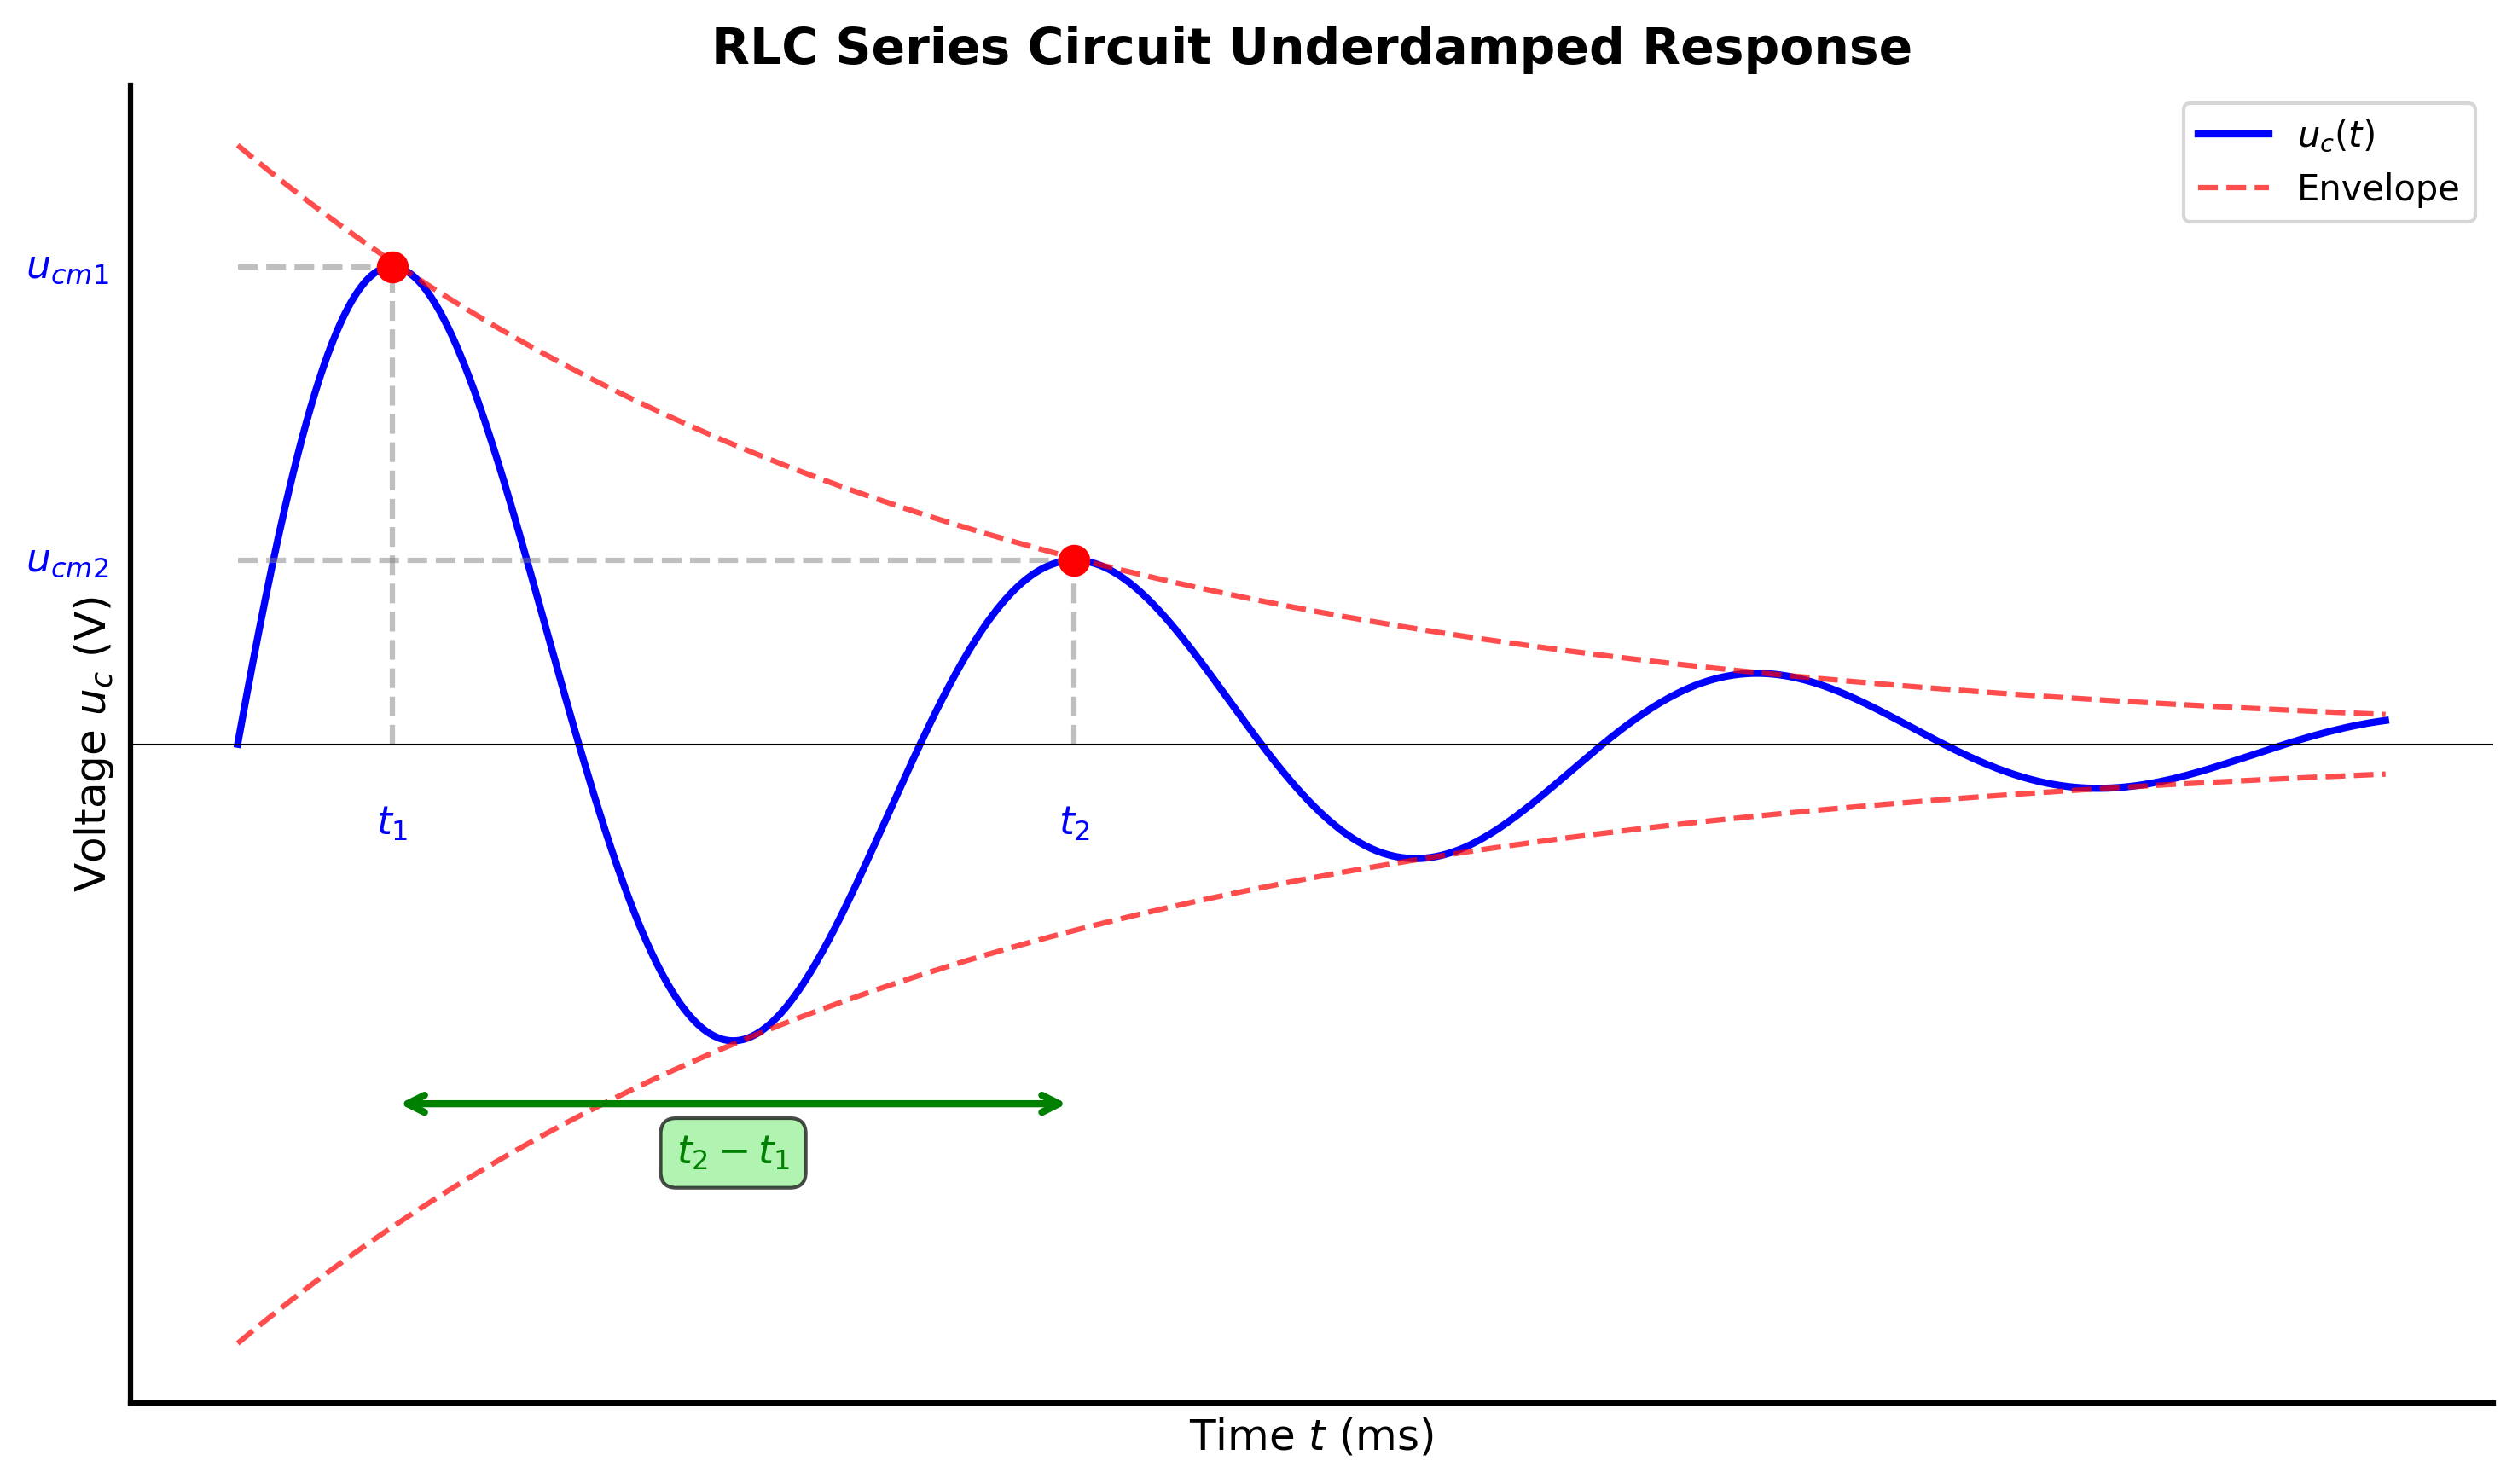
\includegraphics[width=\textwidth]{E10/欠阻尼波形图.png}
        \captionof{figure}{欠阻尼响应波形}
    \end{minipage}
    
    \item \textbf{状态轨迹法}
    
    对于RLC串联电路,也可以在李萨如图形状态下观察,用状态变量/空间轨迹法进行分析。
    
    在整个响应过程中,状态变量随时间连续变化,在状态空间描绘成一条曲线,称之为状态轨迹。将示波器$u_L$从CH1输入,$u_c$从CH2输入,设置X-Y显示方式即可得到状态轨迹。

    \begin{figure}[H]
        \centering
        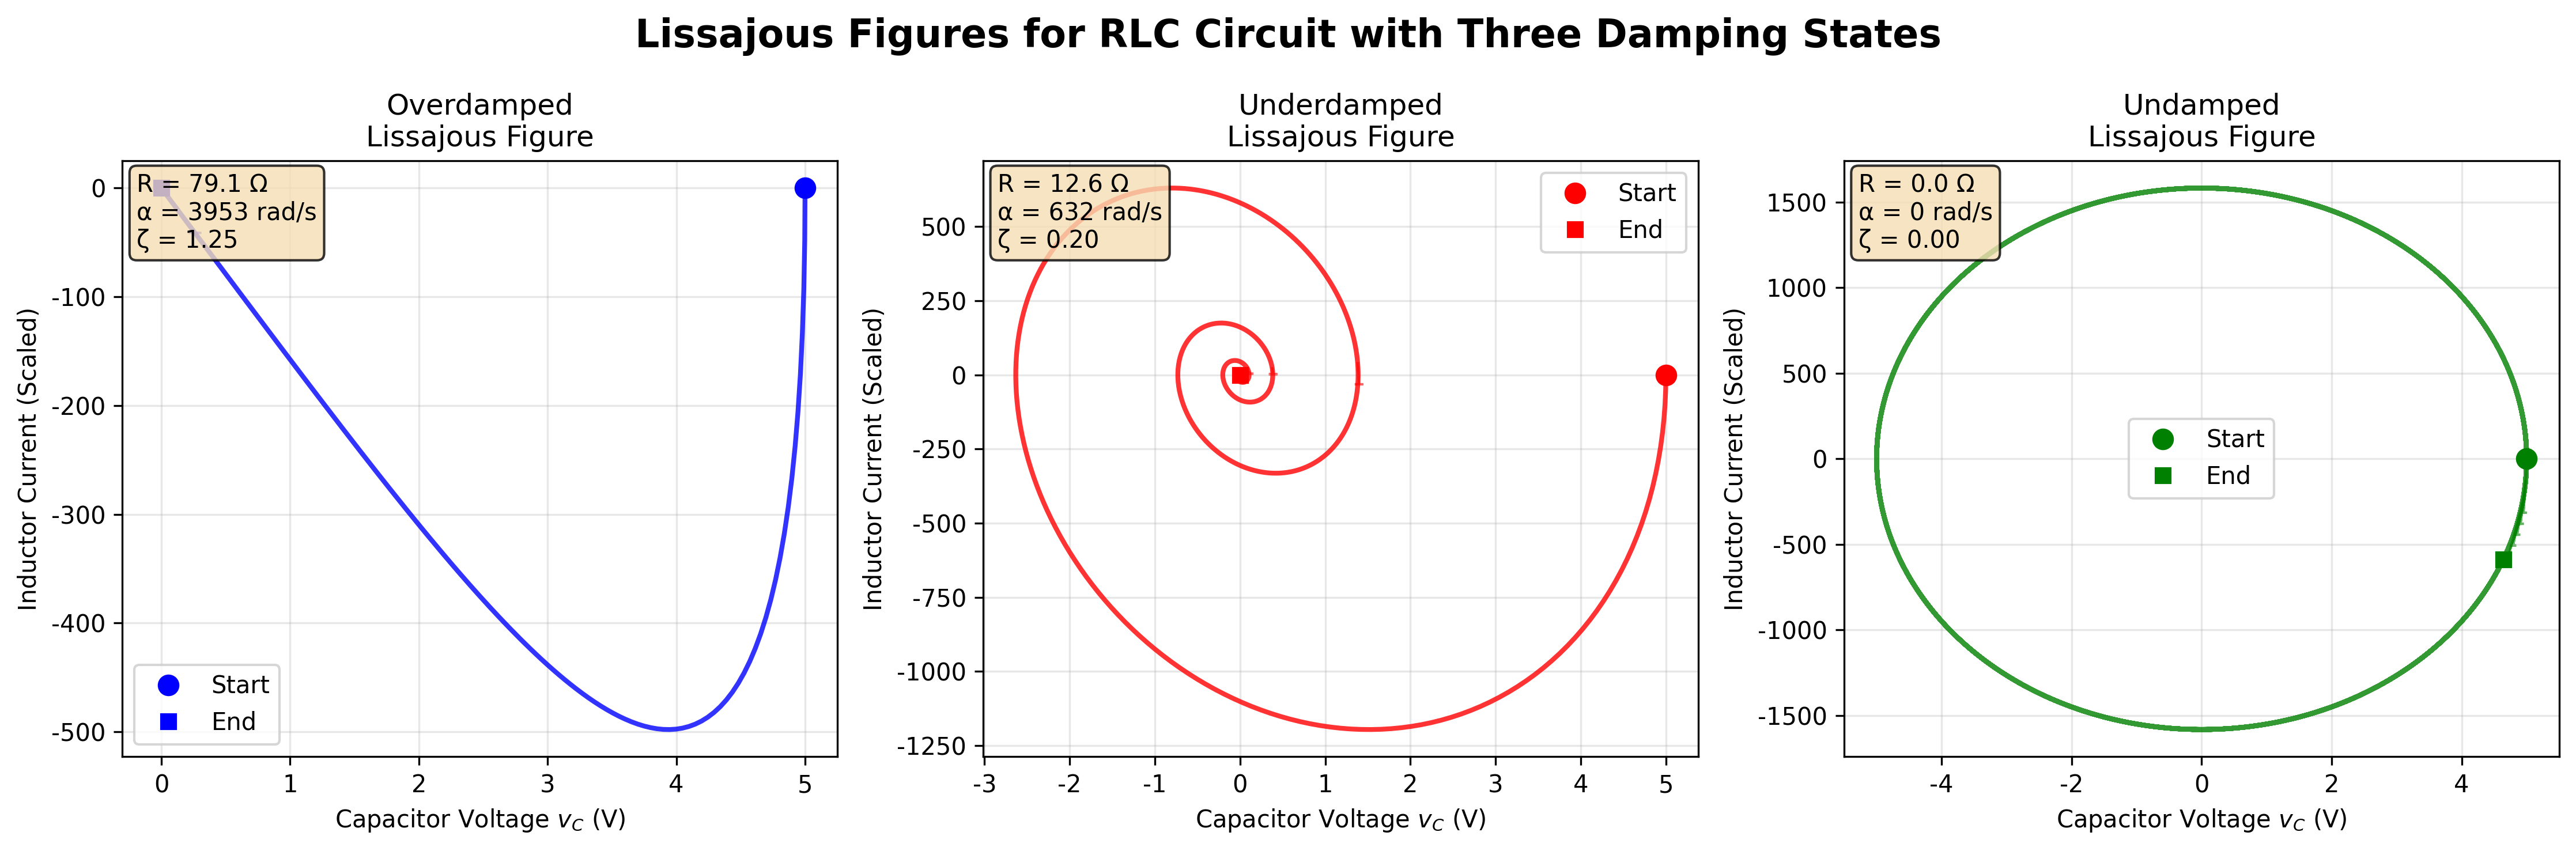
\includegraphics[width=0.95\textwidth]{E10/RLC_Lissajous_Three_Damping_States.png}
        \caption{三种阻尼情况的状态轨迹}
    \end{figure}

\end{enumerate}

\section*{三、思考题}
\begin{enumerate}
    \item 二阶 RLC 串联电路的阻尼系数 $\alpha$ 和固有频率 $\omega_0$ 是否与激励信号有关? 请解释。
    
    \textbf{解：}不相关。
    
    阻尼系数 $\alpha = \dfrac{R}{2L}$ 和固有频率 $\omega_0 = \dfrac{1}{\sqrt{LC}}$ 完全由电路的元件参数决定，与激励信号无关。具体分析如下：
    
    \begin{itemize}
        \item \textbf{阻尼系数$\alpha$}：由电阻R、电感L决定，反映了电路的能量耗散速度。电阻越大或电感越小，阻尼越强。
        
        \item \textbf{固有频率$\omega_0$}：由电感L和电容C决定，反映了电路的固有振荡特性，是LC谐振回路的自然频率。
        
        \item \textbf{激励信号的影响}：激励信号（幅值、频率、波形）只影响响应的幅度和初始条件，不改变电路的固有特性参数。无论激励是阶跃、脉冲还是正弦波，只要元件参数不变，$\alpha$和$\omega_0$就保持不变。
        
        \item \textbf{类比}：这类似于弹簧振子系统，其固有频率和阻尼系数由弹簧劲度和阻尼器特性决定，与外力的大小和形式无关。
    \end{itemize}
    
    因此，$\alpha$和$\omega_0$是电路的\textbf{固有特性参数}，仅取决于电路结构和元件参数，与激励信号无关。
    
        \begin{figure}[H]
        \centering
        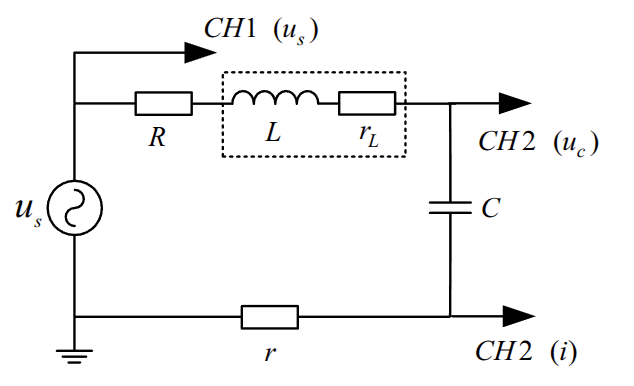
\includegraphics[width=0.5\textwidth]{E10_preview/schematic.png}
        \caption{图 7-18}
    \end{figure}
    
    \item 若把图 7-18 中的电阻 R 和 r 均移除,实验电路是否会出现等幅振荡? 请说明原因。
    
    \textbf{解：}理论上会出现等幅振荡，但实际上不会。
    
    \textbf{理论分析：}
    \begin{itemize}
        \item 移除R和r后，电路中只剩下电感L和电容C，此时总电阻为0（忽略线路和元件内阻）。
        
        \item 阻尼系数变为：$\alpha = \dfrac{0}{2L} = 0$，电路处于\textbf{无阻尼状态}。
        
        \item 在无阻尼条件下（$\alpha = 0$），电路响应为：$u_c(t) = A\sin(\omega_0 t + \varphi)$，即理想LC电路会产生角频率为$\omega_0 = \dfrac{1}{\sqrt{LC}}$的等幅振荡。
        
        \item 能量在电感的磁场能和电容的电场能之间无损耗地来回转换。
    \end{itemize}
    
    \textbf{实际情况：}
    \begin{itemize}
        \item 实际电路中，电感线圈存在\textbf{内阻}$R_L$（铜线电阻），导线也有电阻。
        
        \item 实际阻尼系数：$\alpha = \dfrac{R_L}{2L} > 0$，电路仍有阻尼。
        
        \item 因此实际电路会出现\textbf{衰减振荡}而非等幅振荡，只是衰减速度较慢。
        
        \item 要实现真正的等幅振荡，需要引入\textbf{负阻尼}（如有源补偿电路）来抵消内阻的能量损耗。
    \end{itemize}
    
    \textbf{结论：}理想情况下会等幅振荡，但实际上由于元件固有损耗，只能实现接近等幅的缓慢衰减振荡。

    \item 图 7-18 中的电阻 r 对电流测量结果有何影响吗? 能否改变测量线路来消除其影响? 还有哪些其他可行的补偿方法?
    
    \textbf{解：}电阻r对电流测量有影响，但可以通过多种方法消除或补偿。
    
    \textbf{r的影响：}
    \begin{itemize}
        \item 采样电阻r串联在电路中用于测量电流（通过测量$u_r = i_L \cdot r$来间接测电流）。
        
        \item r会改变电路的总电阻，影响阻尼系数：$\alpha = \dfrac{R + R_L + r}{2L}$，使实际阻尼增大。
        
        \item r上的压降会影响电容和电感上的实际电压分配。
        
        \item 测量值包含了r引入的额外阻尼效应，使测量结果偏离原电路特性。
    \end{itemize}
    
    \textbf{消除影响的方法：}
    
    \textbf{方法一：使用电流探头}
    \begin{itemize}
        \item 采用\textbf{霍尔电流传感器}或\textbf{电流钳}直接测量电流，无需串联采样电阻。
        \item 优点：完全不改变原电路，测量准确。
        \item 缺点：需要专用设备，成本较高。
    \end{itemize}
    
    \textbf{方法二：使用极小阻值的采样电阻}
    \begin{itemize}
        \item 选择$r \ll R$（如$r = 1\Omega$，$R = 100\Omega$），使$r$的影响可忽略。
        \item 计算时将r的影响纳入考虑：$\alpha_{measured} = \dfrac{R + R_L + r}{2L}$，$\alpha_{actual} = \dfrac{R + R_L}{2L}$。
    \end{itemize}
    
    \textbf{方法三：软件补偿}
    \begin{itemize}
        \item 测量完成后，在数据处理时将r的影响计算并扣除。
        \item 修正公式：$\alpha_{corrected} = \alpha_{measured} - \dfrac{r}{2L}$。
    \end{itemize}
    
    \textbf{方法四：差分测量}
    \begin{itemize}
        \item 分别测量有r和无r时的电路响应，通过对比消除r的影响。
    \end{itemize}
    
    \textbf{推荐方案：}实际应用中，结合\textbf{方法二和方法三}，即选用小阻值采样电阻并在计算时进行软件补偿，既经济实用又能保证测量精度。
    
    \item 对于阶跃信号激励下的 RLC 串联电路,在保持其他参数不变时,能否通过调整 R 或 L 来加快或减慢衰减速度? 请说明理由。
    
    \textbf{解：}可以，通过调整R或L都能改变衰减速度。
    
    \textbf{理论依据：}
    
    衰减速度由阻尼系数$\alpha = \dfrac{R}{2L}$决定，响应的衰减包络线为$e^{-\alpha t}$。$\alpha$越大，衰减越快；$\alpha$越小，衰减越慢。
    
    \textbf{调整R的影响：}
    \begin{itemize}
        \item \textbf{增大R}：$\alpha$增大 $\Rightarrow$ 衰减加快
        \begin{itemize}
            \item 电阻增大，能量耗散增加，电路达到稳态所需时间缩短。
            \item 极端情况：R足够大时，从欠阻尼转变为过阻尼（$\alpha > \omega_0$），响应不再振荡。
        \end{itemize}
        
        \item \textbf{减小R}：$\alpha$减小 $\Rightarrow$ 衰减减慢
        \begin{itemize}
            \item 电阻减小，能量耗散减少，振荡持续时间延长。
            \item 极端情况：$R \to 0$时，$\alpha \to 0$，接近等幅振荡。
        \end{itemize}
    \end{itemize}
    
    \textbf{调整L的影响：}
    \begin{itemize}
        \item \textbf{减小L}：$\alpha$增大 $\Rightarrow$ 衰减加快
        \begin{itemize}
            \item 电感减小，电路储能能力下降，能量更快被电阻消耗。
            \item 同时$\omega_0 = \dfrac{1}{\sqrt{LC}}$增大，振荡频率提高。
        \end{itemize}
        
        \item \textbf{增大L}：$\alpha$减小 $\Rightarrow$ 衰减减慢
        \begin{itemize}
            \item 电感增大，电路储能能力增强，能量消耗相对缓慢。
            \item 同时$\omega_0$减小，振荡频率降低。
        \end{itemize}
    \end{itemize}
    
    \textbf{实际应用建议：}
    \begin{itemize}
        \item \textbf{调R更方便}：电阻易于更换调节，是最常用的方法。
        \item \textbf{调L需注意}：改变L会同时影响$\alpha$和$\omega_0$，可能改变阻尼类型，需综合考虑。
        \item \textbf{综合调节}：实际设计中常需要同时调整R和L，以达到期望的衰减速度和振荡频率。
    \end{itemize}
    
    \textbf{定量示例：}假设$L = 100mH$，$C = 0.1\mu F$，$\omega_0 = 10^4 rad/s$
    \begin{itemize}
        \item $R = 50\Omega$: $\alpha = 250 rad/s$ （欠阻尼，衰减较慢）
        \item $R = 200\Omega$: $\alpha = 1000 rad/s$ （欠阻尼，衰减较快）
        \item $R = 2000\Omega$: $\alpha = 10000 rad/s$ （临界阻尼，最快非振荡衰减）
    \end{itemize}
    
    \textbf{结论：}通过调整R或L都能有效控制衰减速度，调R最为便捷实用。
    
\end{enumerate}

\section*{四、实验任务与线路}
\begin{enumerate}
    \begin{figure}[H]
        \centering
        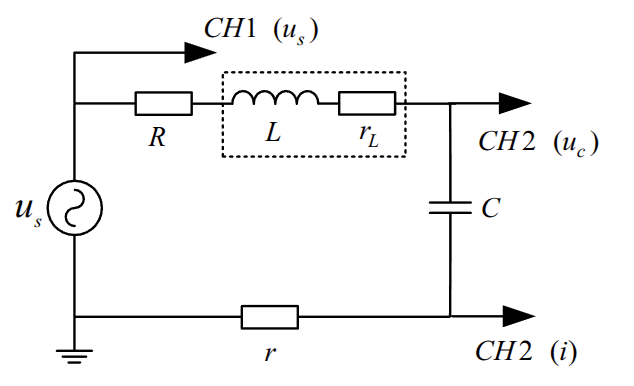
\includegraphics[width=0.5\textwidth]{E10_preview/schematic.png}
        \caption{实验线路图}
    \end{figure}
    \item 按图连接RLC串联二阶电路，在正弦方波激励条件下：$u_s$ = 10V (峰峰值)，$f$ = 200Hz，改变电路中$R$的值，通过观察$u_s$以及$u_c$、$i_L$波形，使电路分别处于过阻尼和欠阻尼状态，并分别记录各自的电阻阻值。

    \item 在过阻尼状态下，先绘制$u_s$、$u_c$、$i_L$的波形（注意体现电路激励和响应的关系），然后绘制$u_c$和$i_L$的状态轨迹。

    \item 在欠阻尼状态下，在同一坐标系绘制$u_s$、$u_c$的波形（或者$u_s$、$i_L$的波形），计算该电路的振荡角频率$\omega_d$和阻尼系数$\alpha$，最后绘制$u_c$和$i_L$的状态轨迹。
\end{enumerate}

\section*{五、实验数据记录与分析}
\subsection*{1.过阻尼状态（$R = 500 \Omega$）}
\begin{figure}[H]
    \centering
    \begin{subfigure}[b]{0.8\textwidth}
        \centering
        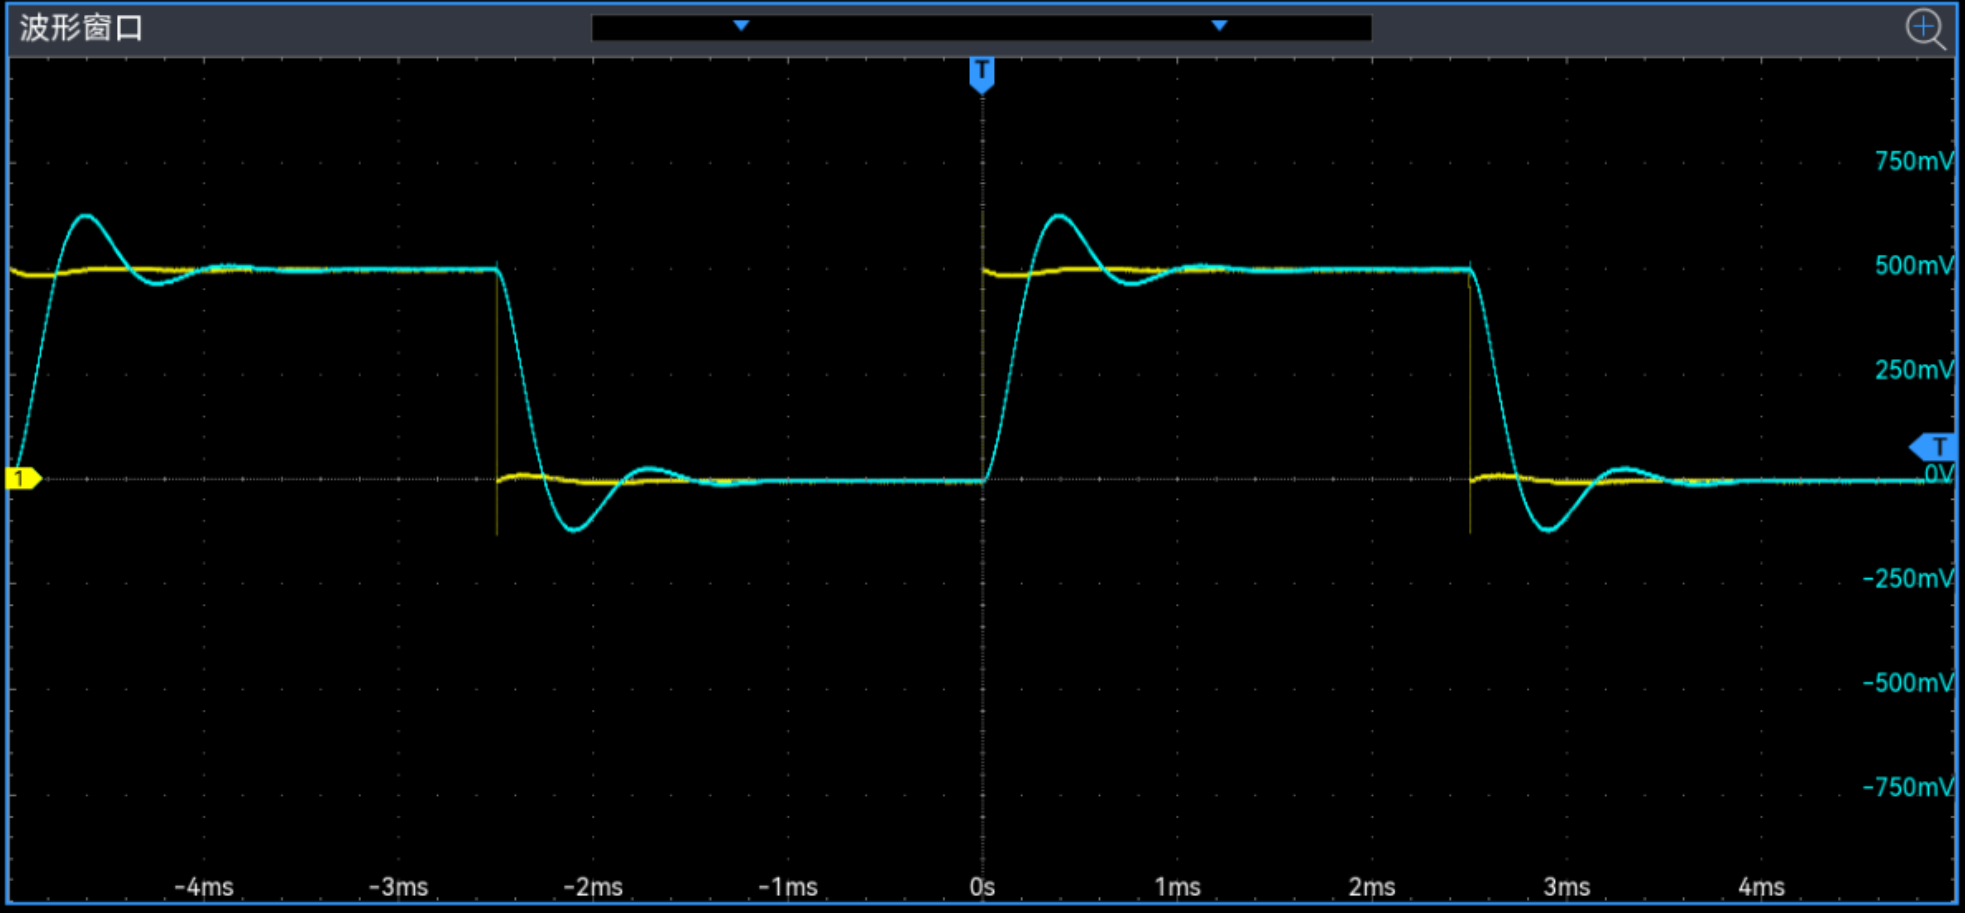
\includegraphics[width=\textwidth]{../picture/overdamping_u.png}
        \caption{过阻尼状态下的电压波形}
        \label{fig:overdamping_u}
    \end{subfigure}
    
    \vspace{0.5cm}
    
    \begin{subfigure}[b]{0.8\textwidth}
        \centering
        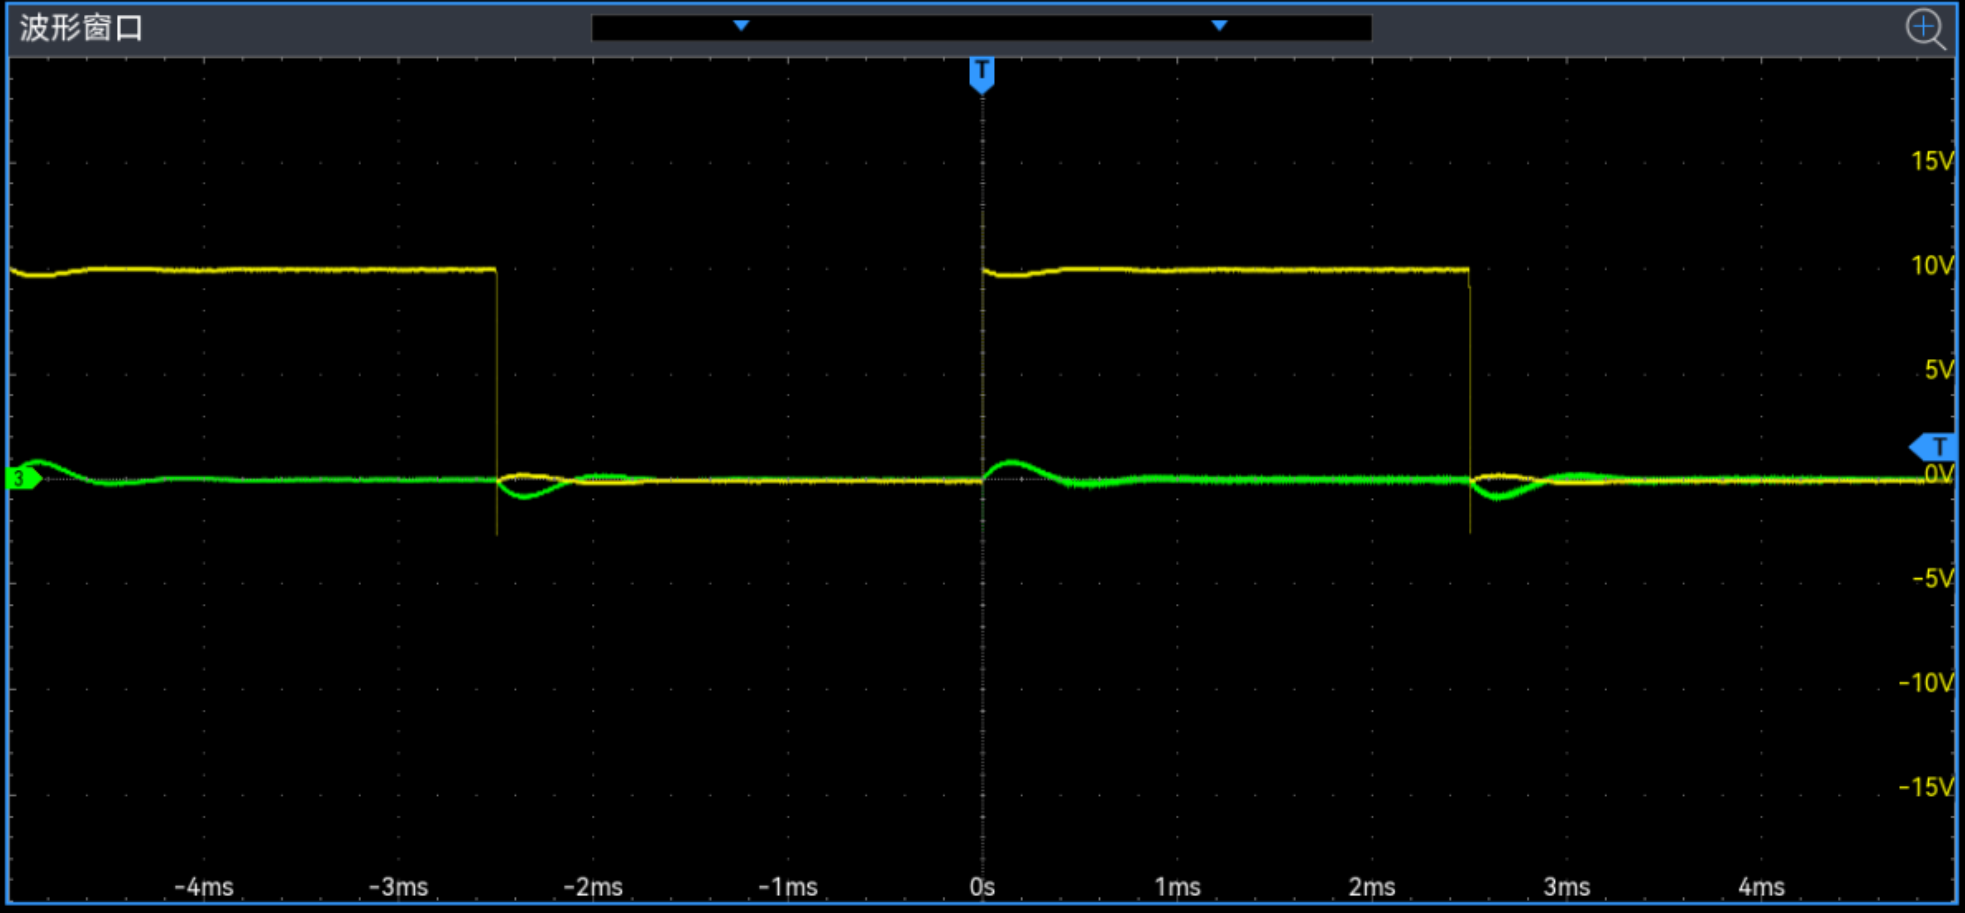
\includegraphics[width=\textwidth]{../picture/overdamping_i.png}
        \caption{过阻尼状态下的电流波形}
        \label{fig:overdamping_i}
    \end{subfigure}
    \caption{过阻尼状态下的电压和电流波形}
    \label{fig:overdamping_waves}
\end{figure}

\textbf{数据记录：}
\begin{itemize}
    \item 电感电阻值：$R_L = 135 \Omega$
    \item 电阻值：$R = 500 \Omega$
    \item 电感值：$L = 100 mH$
    \item 电容值：$C = 0.1 \mu F$
    \item 采样电阻值：$r = 20 \Omega$
\end{itemize}

\textbf{数据分析：}
\begin{itemize}[label={}]
    \item 计算阻尼系数和固有频率：
    \begin{equation*}
        \alpha = \dfrac{R + R_L + r}{2L} = \dfrac{500 + 135 + 20}{2 \times 0.1} = 3275 \si{\per\second}
    \end{equation*}
    \begin{equation*}
        \omega_0 = \dfrac{1}{\sqrt{LC}} = \dfrac{1}{\sqrt{0.1 \times 10^{-3} \times 0.1 \times 10^{-6}}} = 10^5 \si{\per\second}
    \end{equation*}
    \item 由于$\alpha < \omega_0$，电路处于过阻尼状态，符合实验预期。


\begin{figure}[H]
    \centering
    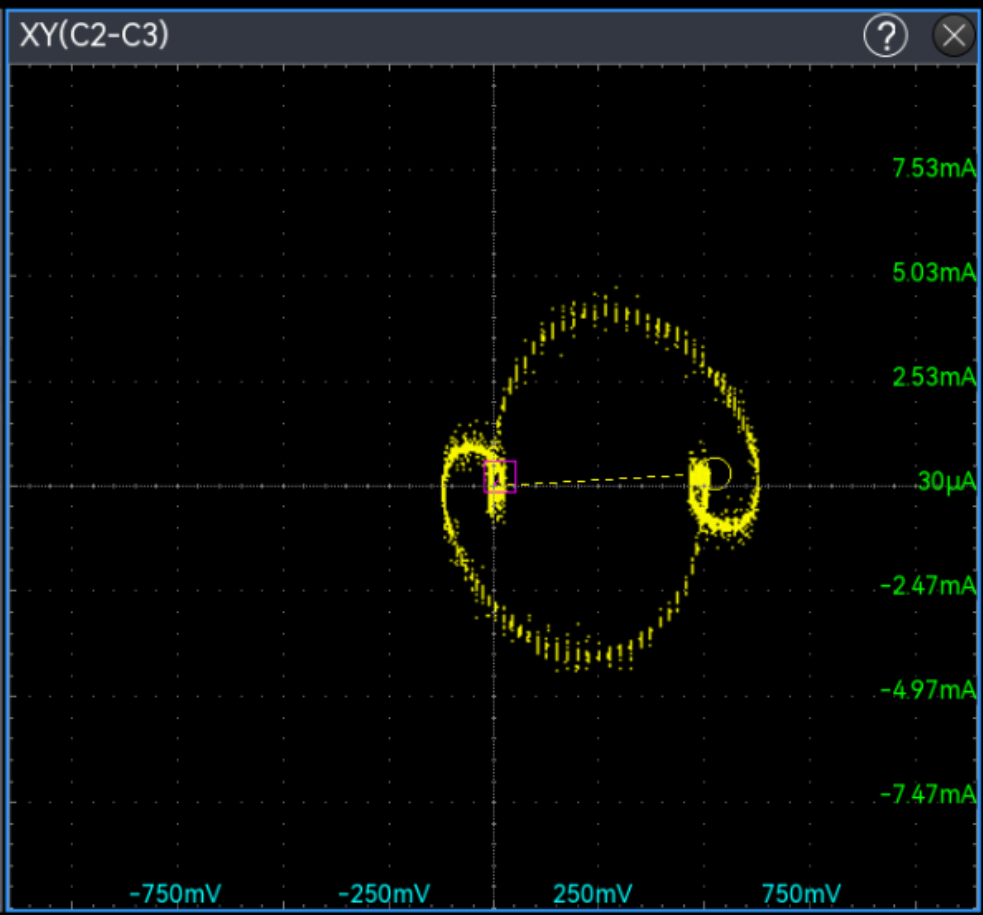
\includegraphics[width=0.6\textwidth]{../picture/overdamping_lissajous.png}
    \caption{过阻尼状态下的状态轨迹}
    \label{fig:overdamping_phase}
\end{figure}

    \item 过阻尼状态下的状态轨迹分析：
    \begin{itemize}
        \item \textbf{轨迹形状}：过阻尼状态的轨迹呈现\textbf{椭圆形}或\textbf{类椭圆形}，直接从初始状态收敛至原点，不发生振荡。
        
        \item \textbf{运动方向}：轨迹发展方向为\textbf{顺时针}，这是因为电感电流$i_L$相位滞后于电容电压$u_C$。在RLC串联电路中，电流变化总是滞后于电压变化。
        
        \item \textbf{收敛特性}：轨迹单调地向原点收敛，无振荡和超调，这是过阻尼系统的典型特征。由于阻尼很强（$\alpha > \omega_0$），系统能量被快速耗散。
        
    \end{itemize}
    
\end{itemize}

\subsection*{2.欠阻尼状态（$R = 100 \Omega$）}
\begin{figure}[H]
    \centering
    \begin{subfigure}[b]{0.8\textwidth}
        \centering
        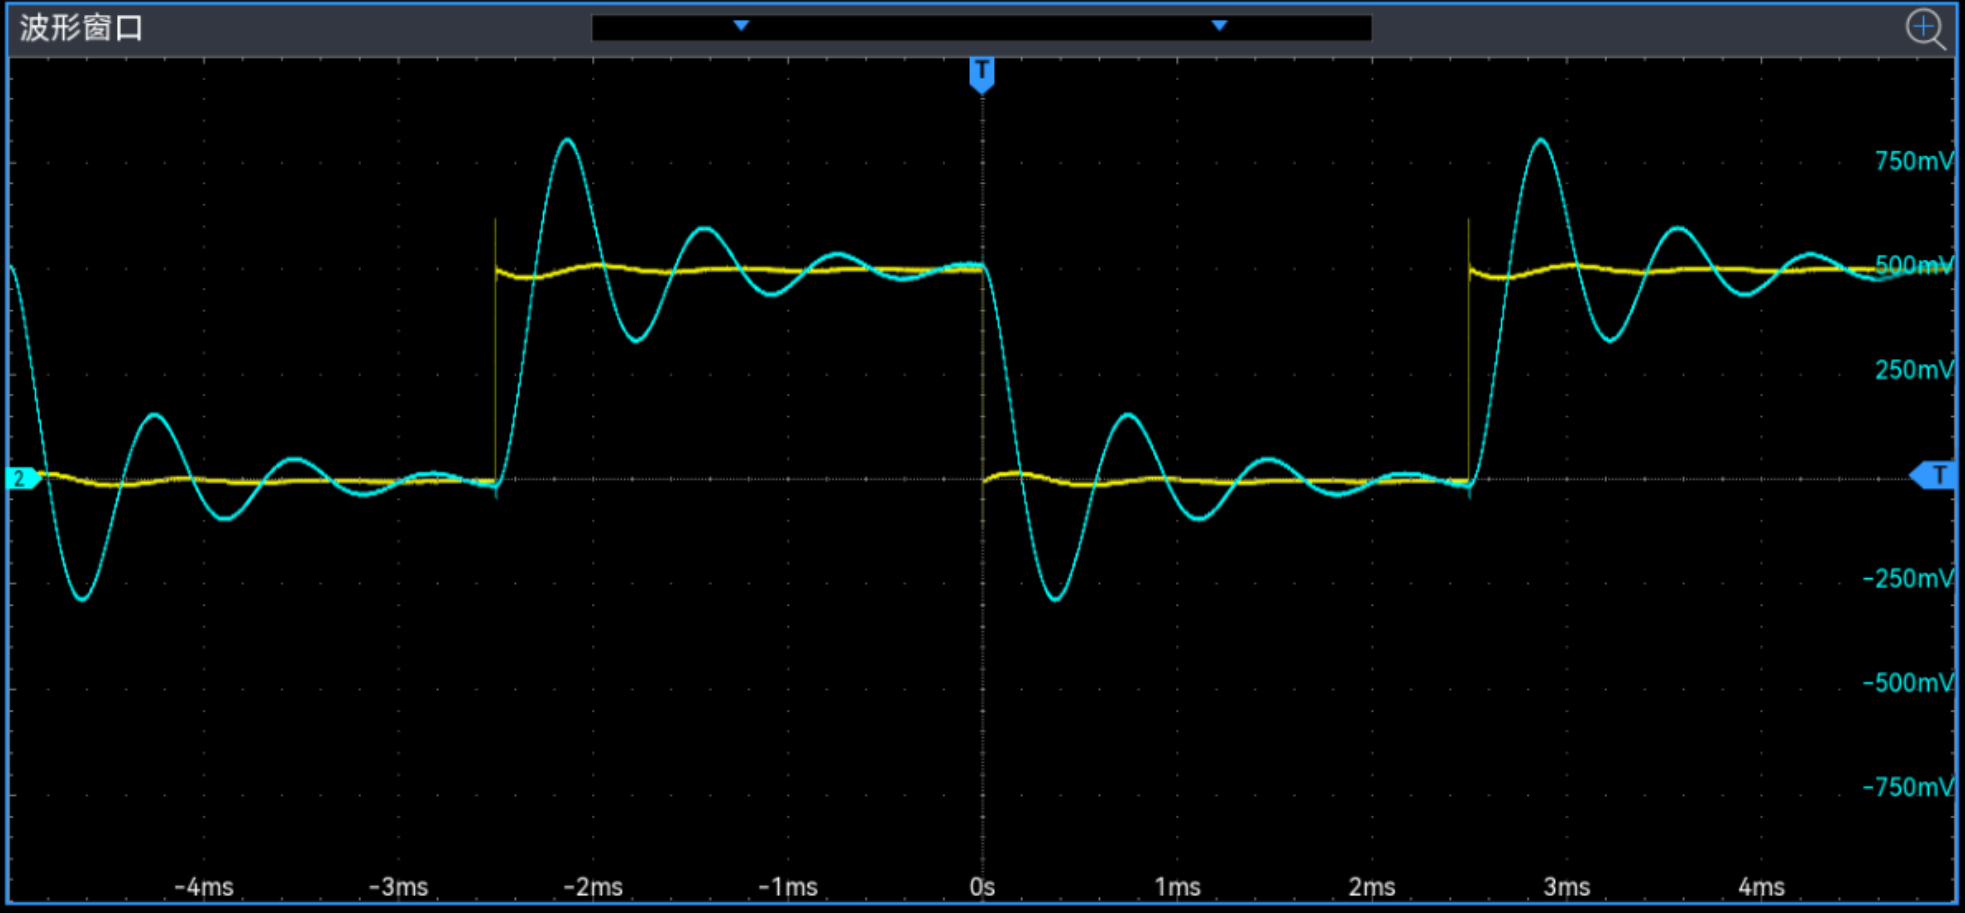
\includegraphics[width=\textwidth]{../picture/underdamping_u.png}
        \caption{欠阻尼状态下的电压波形}
        \label{fig:underdamping_u}
    \end{subfigure}
    
    \vspace{0.5cm}
    
    \begin{subfigure}[b]{0.8\textwidth}
        \centering
        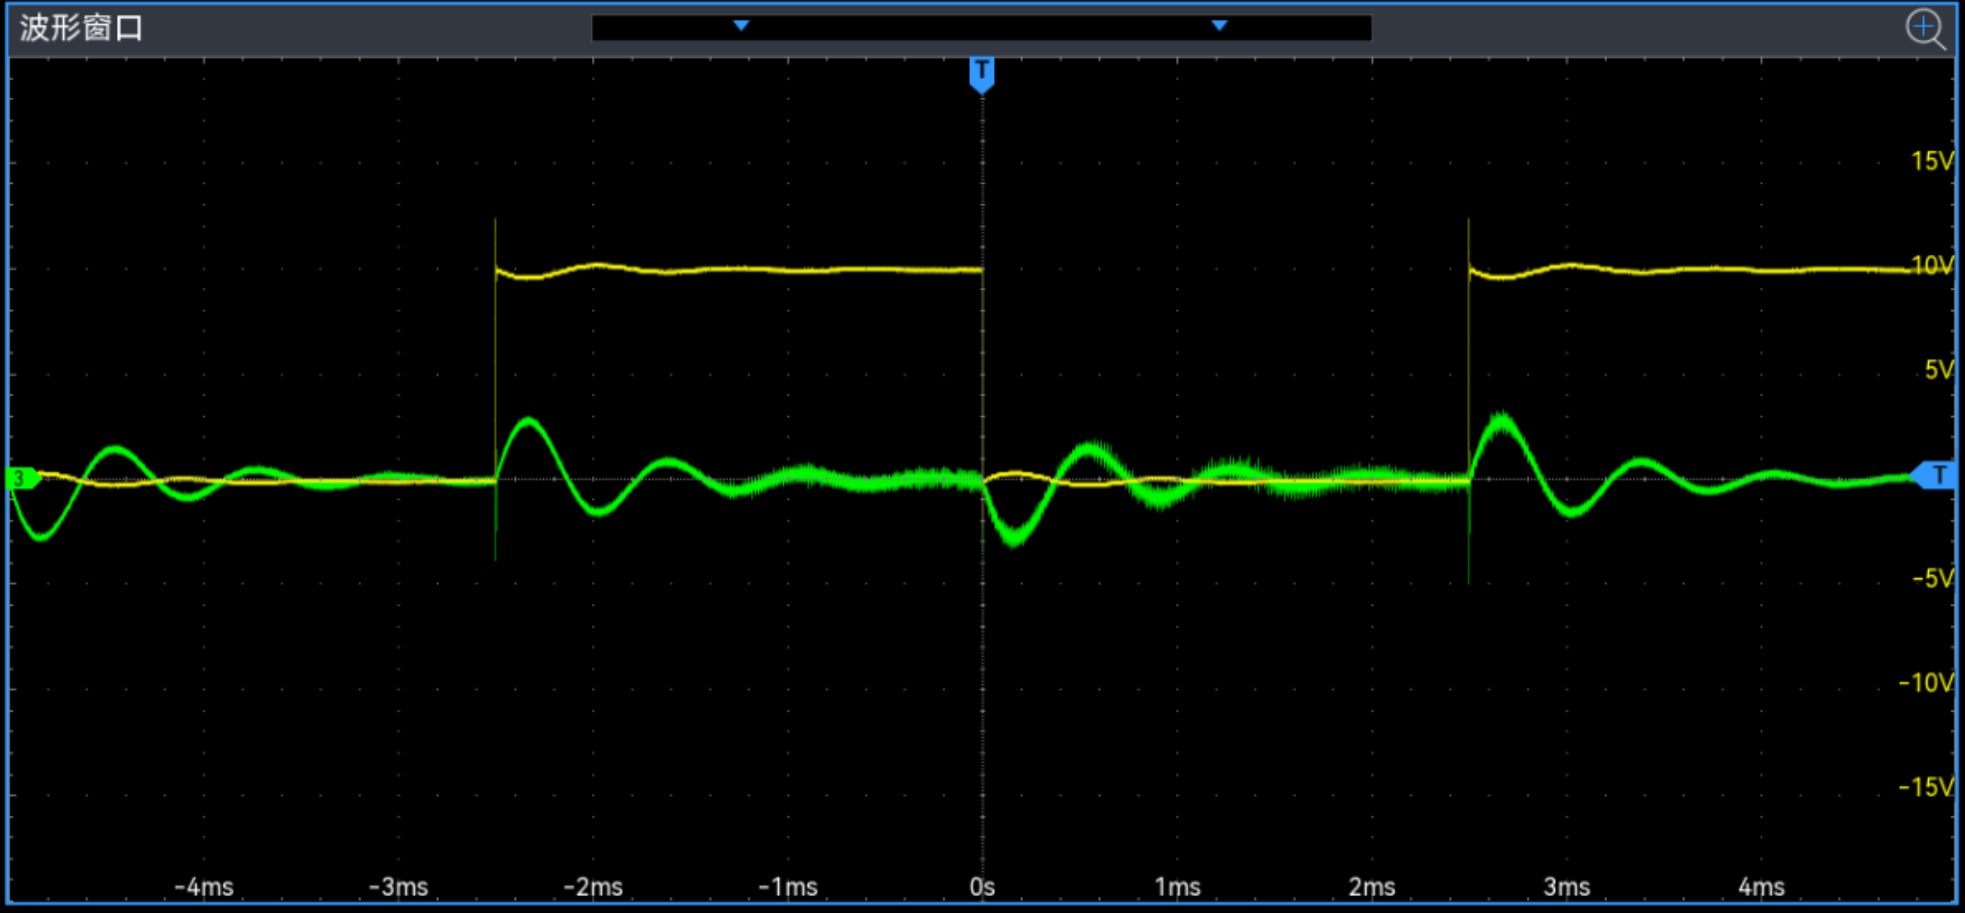
\includegraphics[width=\textwidth]{../picture/underdamping_i.png}
        \caption{欠阻尼状态下的电流波形}
        \label{fig:underdamping_i}
    \end{subfigure}
    \caption{欠阻尼状态下的电压和电流波形}
    \label{fig:underdamping_waves}
\end{figure}

\textbf{数据记录：}
\begin{itemize}
    \item 电感电阻值：$R_L = 135 \Omega$
    \item 电阻值：$R = 100 \Omega$
    \item 电感值：$L = 100 mH$
    \item 电容值：$C = 0.1 \mu F$
    \item 采样电阻值：$r = 20 \Omega$
    \item 阻尼峰值：$u_{cm1} = -266.87 mV, u_{cm2} = -109.95 V$
    \item 峰值时间间隔：$t_1 = 0.384 ms, t_2 = 1.055 ms$
\end{itemize}

\textbf{数据分析：}
\begin{itemize}[label={}]
    \item 计算阻尼系数和固有频率：
    \begin{equation*}
        \alpha = \dfrac{R + R_L + r}{2L} = \dfrac{100 + 135 + 20}{2 \times 0.1} = 1275 \si{\per\second}
    \end{equation*}
    \begin{equation*}
        \omega_0 = \dfrac{1}{\sqrt{LC}} = \dfrac{1}{\sqrt{100 \times 10^{-3} \times 0.1 \times 10^{-6}}} = 10^4 \si{\per\second}
    \end{equation*}
    \item 由于$\alpha < \omega_0$，电路处于欠阻尼状态，符合实验预期。
    \item 计算振荡角频率和阻尼系数：
    \begin{equation*}
        \omega_d = \dfrac{2\pi}{t_2 - t_1} = \dfrac{2\pi}{1.105 \times 10^{-3} - 0.384 \times 10^{-3}} = 9.364 \times 10^{3} \si{\per\second}
    \end{equation*}
    \begin{equation*}
        \alpha = \dfrac{1}{t_2 - t_1} \ln\left(\dfrac{u_{cm1}}{u_{cm2}}\right) = \dfrac{1}{1.105 \times 10^{-3} - 0.384 \times 10^{-3}} \ln\left(\dfrac{-266.87 \times 10^{-3}}{-109.95 \times 10^{-3}}\right) = 1.230 \times 10^{3} \si{\per\second}
    \end{equation*}
        \item 计算相对误差：
    \begin{equation*}
        U_r(\omega) = \left|\dfrac{\omega_{measured} - \omega_{theoretical}}{\omega_{theoretical}}\right|=  \left|\dfrac{9364 - 10000}{10000}\right| = 6.36\%
    \end{equation*}
    \begin{equation*}
        U_r(\alpha) = \left|\dfrac{\alpha_{measured} - \alpha_{theoretical}}{\alpha_{theoretical}}\right|= \left|\dfrac{1275 - 1230}{1275}\right| = 3.53\%
    \end{equation*}
    \item 计算结果与理论值基本一致，验证了实验的正确性。

\begin{figure}[H]
    \centering
    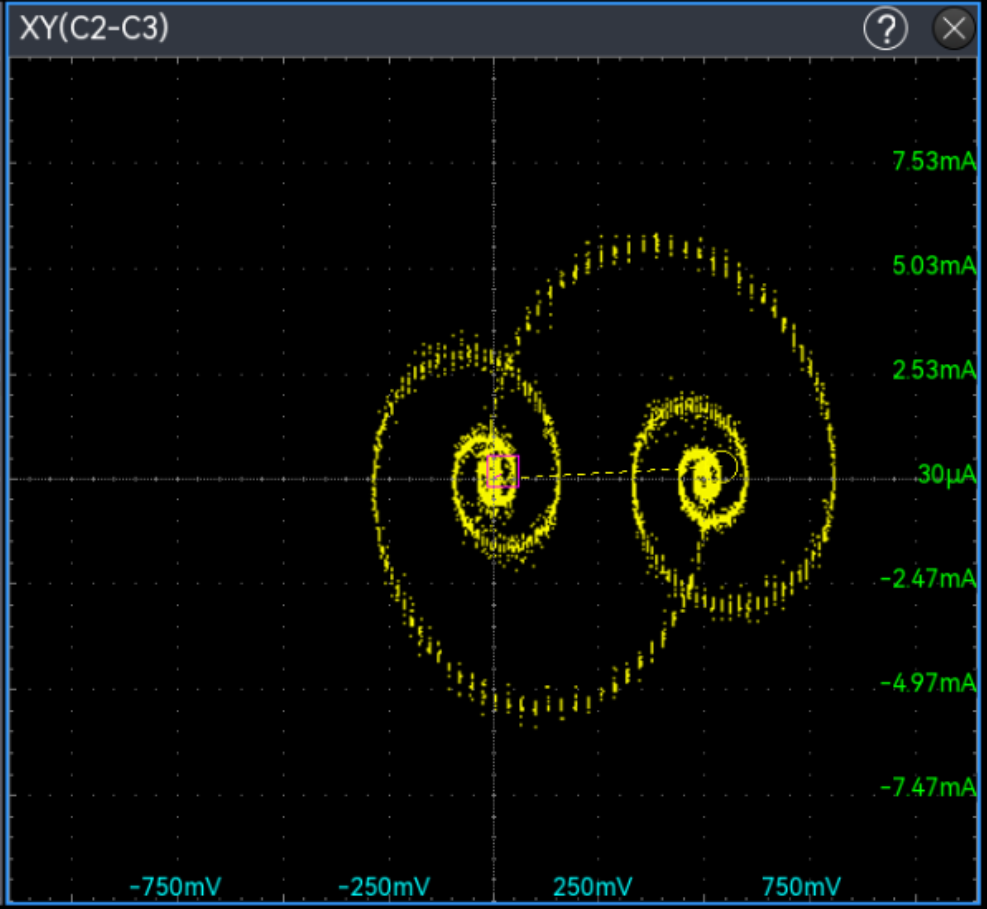
\includegraphics[width=0.6\textwidth]{../picture/underdamping_lissajous.png}
    \caption{欠阻尼状态下的状态轨迹}
    \label{fig:underdamping_phase}
\end{figure}

    \item 欠阻尼状态下的状态轨迹分析：
    \begin{itemize}
        \item \textbf{轨迹形状}：欠阻尼状态的轨迹呈现\textbf{螺旋形}，从外向内逐渐收敛至原点，这是典型的欠阻尼二阶系统特征。
        
        \item \textbf{运动方向}：轨迹发展方向为\textbf{顺时针}，这是因为在RLC串联电路中，电感电流$i_L$相位滞后于电容电压$u_C$。
        
        \item \textbf{收敛特性}：螺旋轨迹向原点收敛，表明系统能量在振荡过程中不断被电阻消耗，最终达到稳态（原点）。螺旋的疏密程度反映了阻尼的大小，阻尼越小，螺旋越密集。
        
        \item \textbf{周期性}：相邻螺旋圈对应一个振荡周期$T_d = \dfrac{2\pi}{\omega_d}$，从图中可以直观看出振荡的衰减过程。
        
        \item \textbf{与过阻尼对比}：与过阻尼状态的椭圆轨迹不同，欠阻尼的螺旋轨迹反映了系统的振荡性质，说明系统在能量耗散的同时伴随着周期性的能量交换。
    \end{itemize}
    
\end{itemize}

\section*{六、实验小结}
通过本次实验，我深入了解了RLC串联二阶电路的响应过程和基本原理。实验中，我学习并掌握了测量RLC串联二阶电路状态轨迹的方法，以及利用示波器测量衰减振荡的角频率和阻尼系数的技术。

在实验过程中，我观察到了二阶电路在不同阻尼情况下的响应特性：过阻尼时电路响应呈非振荡性衰减，欠阻尼时呈现衰减振荡特性。通过改变电阻值，我亲身体验了电路参数对响应形式的影响，加深了对阻尼系数$\alpha = \dfrac{R}{2L}$和固有频率$\omega_0 = \dfrac{1}{\sqrt{LC}}$物理意义的理解。

此外，通过绘制状态轨迹图，我直观地认识到了状态空间分析方法的优势，这种方法能够清晰地展现电路状态变量之间的动态关系。本次实验不仅巩固了理论知识，也提高了我使用示波器进行精确测量和数据分析的能力。

\end{document}